\tqt{One advantage which Welsh law enjoyed in the political storms of the thirteenth century was that it had a written form. Already in the twelfth century it was felt to be an embarassment if law remained unwritten. Roman law was embodied in texts, and with the great legal revival of the eleventh and twelfth centuries it was felt that any law worthy of the name should be written.
}{charles-edwards_welsh_1989}{14}

\tqt{Welsh law survives in many complete manuscripts and fragments of others. The difficulty scholars have had in coping with this wealth of material stems from two opposite truths: first, each manuscript is an individual entity in that no one manuscript presents a text exactly the same as any other; but, secondly, the manuscripts fall into groups because they share, to a greater or lesser extent, the same content. As a result there have been long terminological travails attempting to give due weight both to the variations between manuscripts and also the links between them.
}{charles-edwards_welsh_1989}{17}


\tqt{The considerable differences between the law books show that their authors were not concerned, like the Irish, to preserve intact a standard text handed down from the past.
  Linguistically, the laws are not unlike many Middle Welsh prose tales: in spite of the occasional early feature the language as a whole generally acords with the dates of the manuscripts.
}{charles-edwards_welsh_1989}{21--22}

\tqt{{[T]}he distinction between the Versions [\eg of Gwynedd, Deheubarth, Gwent] and the Anomalous Laws lies in the existence of a certain pattern according to which it was thought that a wide-ranging account of the Law of Hywel ought to be constructed. The pattern was not immutable, as is shown by the creation of the Test Book in \textsc{Ior} or by the wide variations in the ordering of the tractates in \textsc{Cyfn}.}{charles-edwards_welsh_1989}{26}

\begin{figure}[h]
  \centering
  \begin{tabular}{cc}
I  & II\\
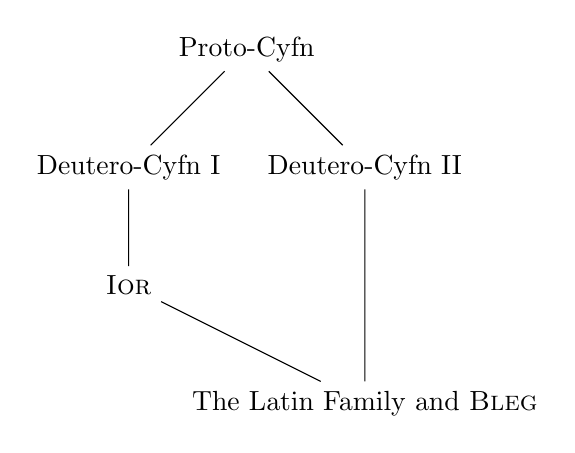
\begin{tikzpicture}[level distance=15mm]
\node(p){Proto-Cyfn}
child{node {Deutero-Cyfn I}
  child{node(ior){\textsc{Ior}}}
}
child[missing]
child {node {Deutero-Cyfn II}
  child[level distance=30mm] {node(lat){The Latin Family and \textsc{Bleg}}}
}
;
\draw(ior)--(lat);    
\end{tikzpicture}
   &
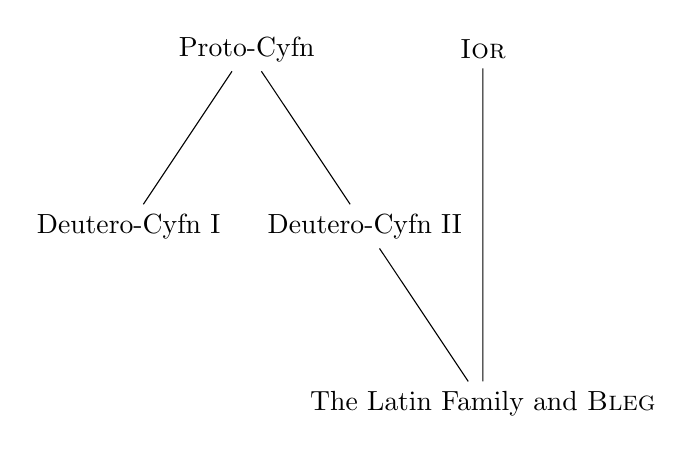
\begin{tikzpicture}[level distance=22.5mm]
\node(p){Proto-Cyfn}
child{node {Deutero-Cyfn I}
}
child[missing]
child {node {Deutero-Cyfn II}
  child[xshift=15mm] {node(lat){The Latin Family and \textsc{Bleg}}}
}
;
\node[xshift=30mm](ior){\vphantom{J}\textsc{Ior}};
\draw(ior)--(lat);
\end{tikzpicture}
\end{tabular}

\caption{Two possible family trees of the Welsh law books according to \textcite[48]{charles-edwards_welsh_1989}.}
\label{fig:lawfamilies}
\end{figure}

\begin{table}[h]
  \centering
  \begin{tabular}{@{}ll@{}}
    \toprule
    \tch{Old} & \tch{New} \\
    \midrule
    Ɛ & Ep \\
    Ð & Dd \\
    Ā & As\\
    \rotatebox[origin=c]{180}{ω}& Mor\\
     & An \\
    \bottomrule
  \end{tabular}
\caption{Sigla for the anomalous laws}
\label{tab:sigla}
\end{table}

\begin{table}[h]
\centering
  \renewcommand{\labelenumi}{\Roman{enumi}}
  \renewcommand{\labelenumii}{\arabic{enumii}}
  \renewcommand{\labelenumiii}{(\roman{enumiii})}
\begin{tabular}{@{}p{0.45\textwidth}p{0.45\textwidth}@{}}
  \toprule
  \tch{\itshape Mk:}&\tch{\textsc{Ior}:}\\\midrule
\begin{enumerate}
\item Prologue
\item Laws of Court
\item Laws of Country
  \begin{enumerate}
  \item The Three Columns of Law, the Nine Tongued-ones, the value of limbs, \mw{galanas} and \mw{sarhaed}
  \item Land
  \item Value of Wild and Tame
  \item Other Laws of Country
    \begin{enumerate}
    \item Corn-damage
    \item Suretyship
    \item Women
    \end{enumerate}
  \end{enumerate}
\item Triads
\end{enumerate}
&

\begin{enumerate}
\item Prologue
\item The Book of the Court (43/17 from Manuscript \textit{B})
\item The Laws of Country
  \begin{enumerate}
  \item The Nine Tongued-ones
  \item Women
  \item Injury to Animals
  \item Surety and Contract
  \item Church Protection
  \item Land
  \item Children and Paternity
  \end{enumerate}
\item The Test Book (colophon: 120/7)
  \begin{enumerate}
  \item The Three Columns of Law (colophon: 120/7)
  \item Value of Wild and Tame (and the Value of Trees)
  \end{enumerate}
\item Appendages to the Test Book:
  \begin{enumerate}
  \item Value of Houses and Equipment
  \item Joint-ploughing
  \item Corn-damage
  \end{enumerate}
\end{enumerate}\\\bottomrule
\end{tabular}
\caption{The main divisions of \textit{Mk} and \textsc{Ior} according to \textcite[27--28]{charles-edwards_welsh_1989}}
\label{tab:divisions}
\end{table}



%%% Local Variables:
%%% mode: latex
%%% coding: utf-8
%%% TeX-master: "../main"
%%% End:
